\documentclass{standalone}

% Font
\usepackage{mathpazo}
\usepackage{libertine}
\renewcommand*\sfdefault{phv}

\large

% Color
\usepackage{xcolor}
\definecolor{f1}{HTML}{F39019}
\definecolor{b1}{HTML}{DE6A10}
\definecolor{f2}{HTML}{51A7F9}
\definecolor{b2}{HTML}{0365C0}
\definecolor{f3}{HTML}{70BF41}
\definecolor{b3}{HTML}{00882B}

% tikz
\usepackage{tikz}
\tikzstyle{every node}=[font=\sffamily]
\usetikzlibrary{shapes,arrows,positioning,calc,decorations.markings,backgrounds}
\tikzstyle{c1} = [thick,draw=b1,fill=f1]
\tikzstyle{c2} = [thick,draw=b2,fill=f2]
\tikzstyle{c3} = [thick,draw=b3,fill=f3]
\tikzstyle{cg} = [thick,draw=gray!50,fill=gray!30]
\tikzstyle{rect} = [rectangle, minimum height=1cm]
\tikzstyle{roundrect} = [rect, rounded corners=.2cm]
\tikzstyle{io} = [trapezium, trapezium left angle=70, trapezium right angle=110]
\tikzstyle{arrow} = [thick,->,>=stealth]

\tikzstyle{ma}=[-stealth, line width=2pt, f3]

\begin{document}
	
\begin{tikzpicture}

\begin{scope}[xshift=1.5cm]
\node[anchor=south west,inner sep=0] (image) at (0,0) {
	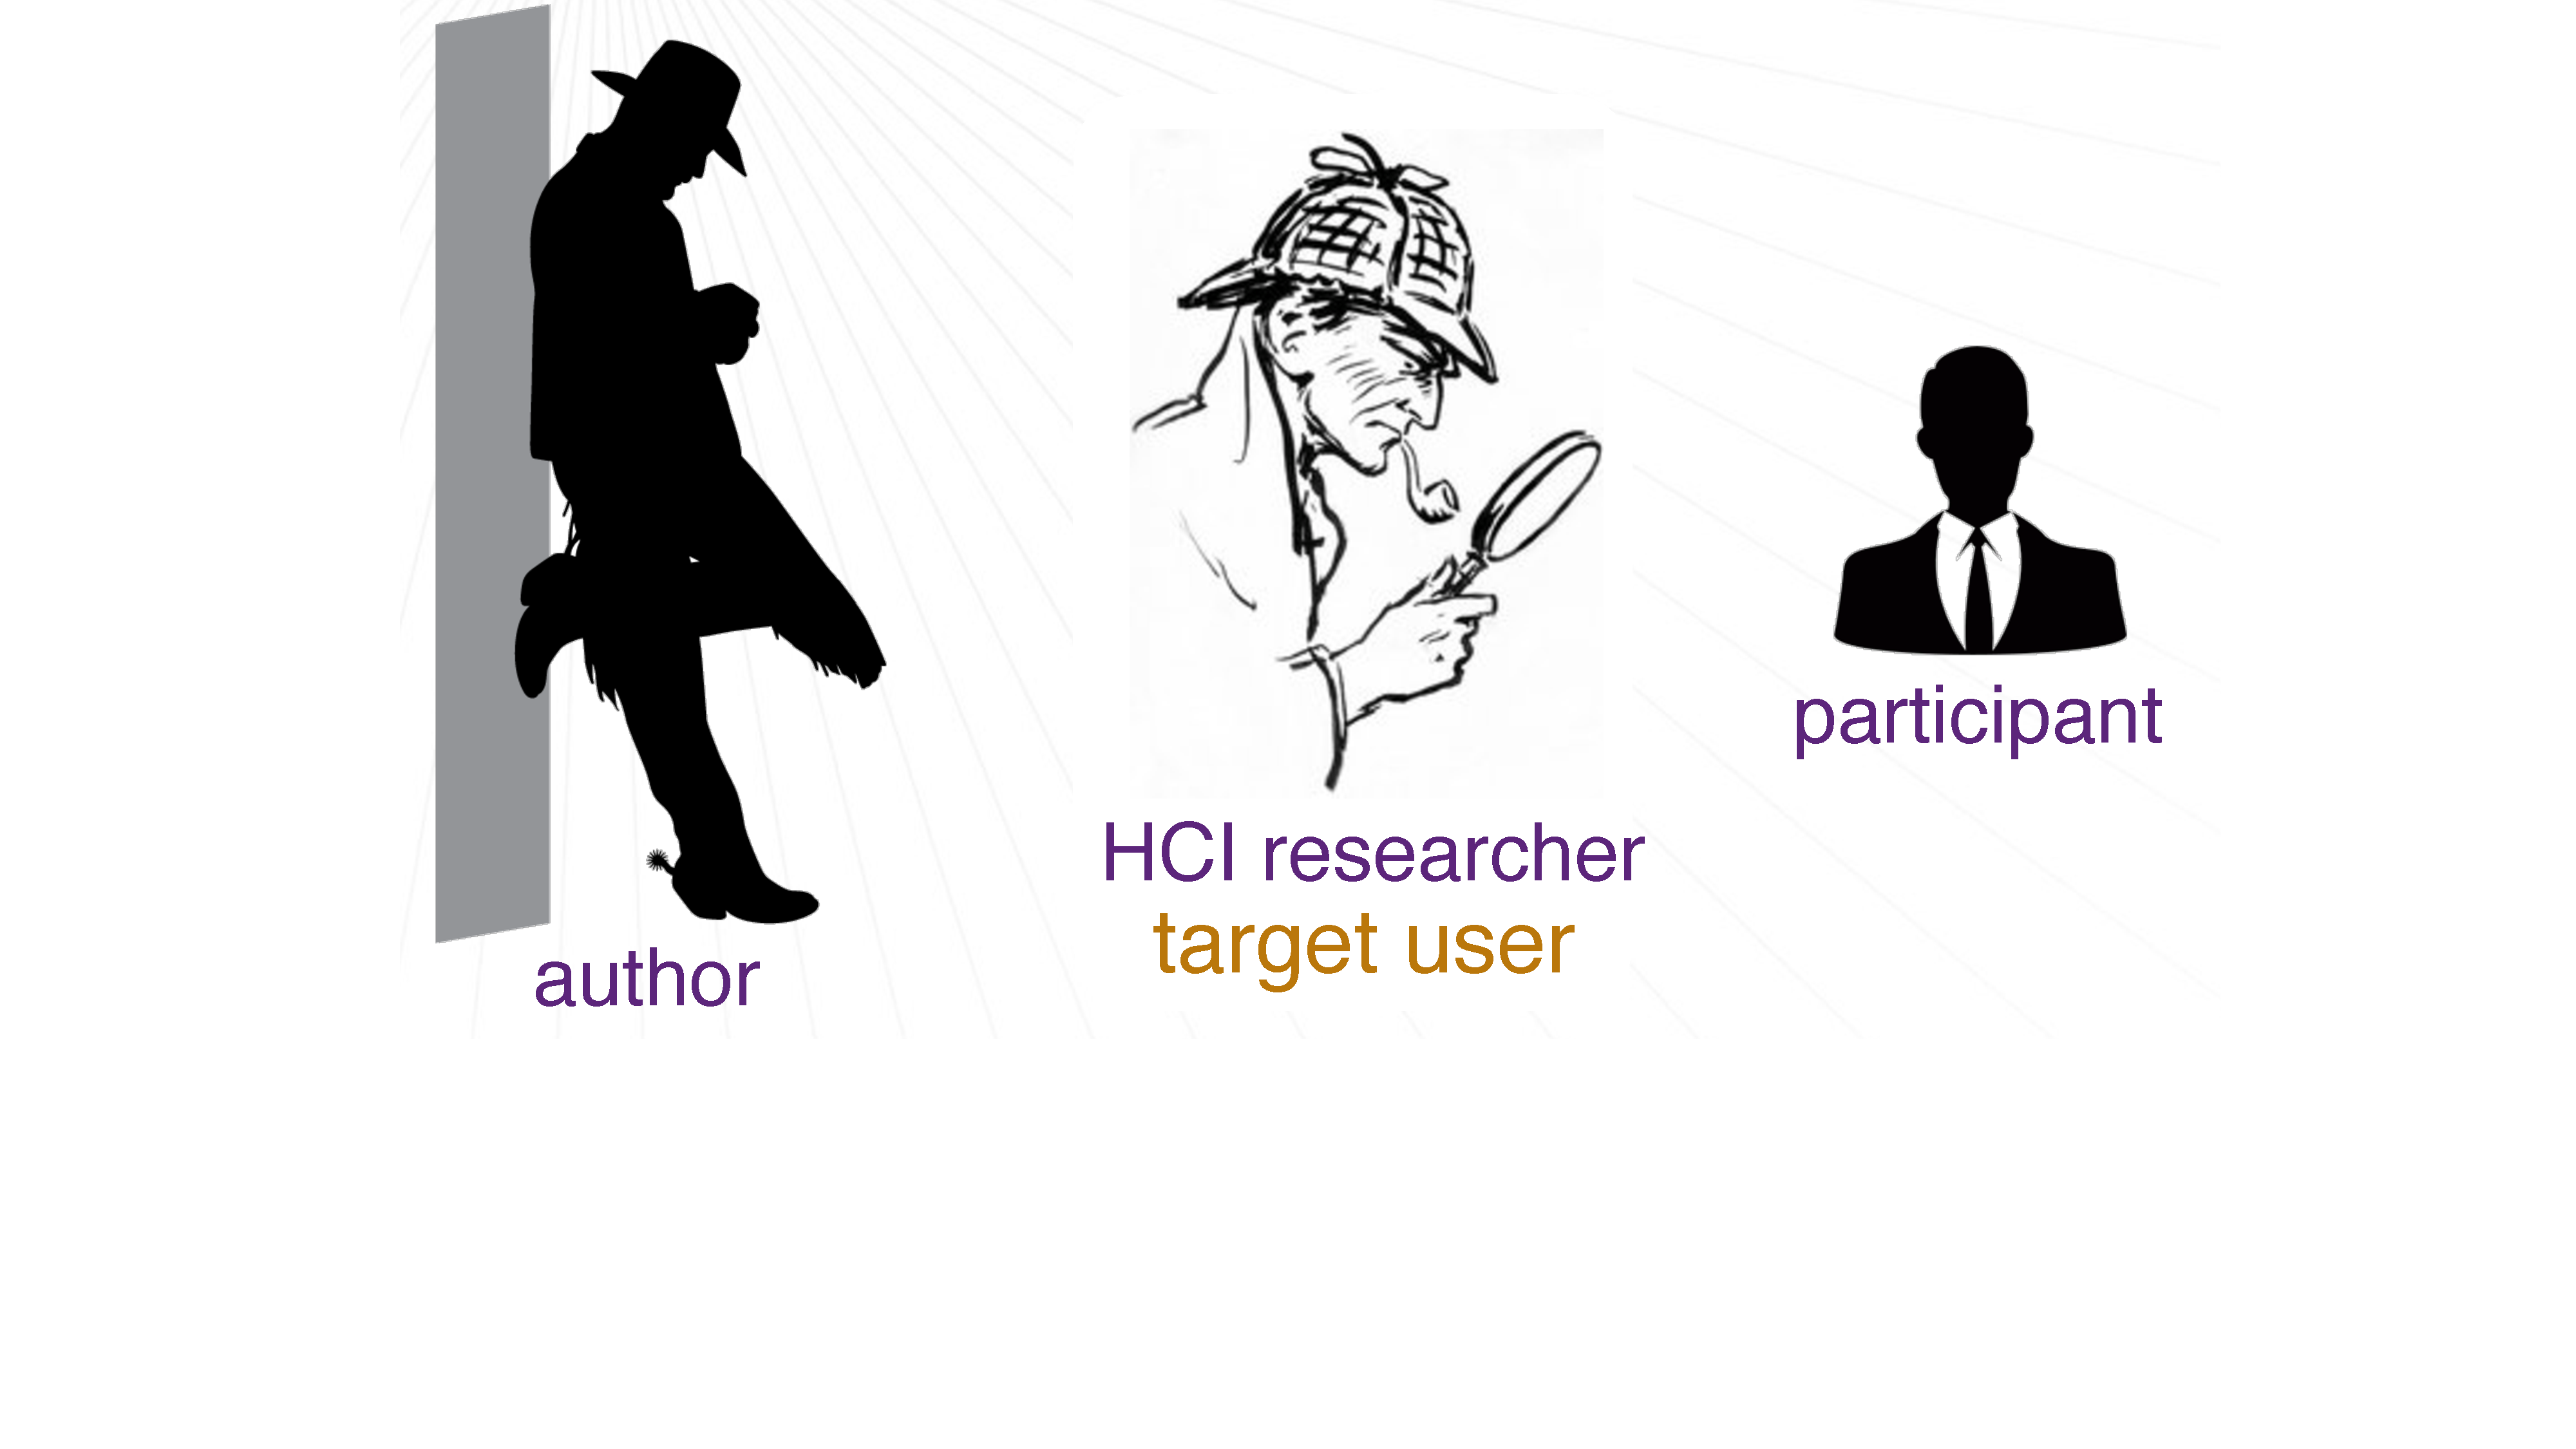
\includegraphics[width=0.35\linewidth]{user-definition}
};

\begin{scope}[x={(image.south east)},y={(image.north west)}]
\draw [ma] (.25,.55) -- ++(.1,0);
\draw [ma] (.7,.55) -- ++(.1,0);
\end{scope}
\end{scope}

\end{tikzpicture}

\end{document}